In this chapter, the ups and downs of the report will be covered and the quality of the tests and data acquired will be evaluated. Moreover, the unimplemented features will be discussed, as well as the requirements and methods for possible implementation.
\section{Ultrasonic Sensors}
The rangefinders have been tested to work quite well - their detection range is reasonable for a drone and their performance speed is excellent. However, if the sensor does not get back the signal it sent out, the $NewPing$ library will return the distance as 0 $cm$ - which is logical in a sense that it lets the user know there was a problem. It should be noted, though, that due to the nature of ultrasonic sensors, receiving the returning signal can be difficult in cases where the object's surface is uneven or it otherwise distorts the soundwave. Thus, while in flight, the sensors could read 0 $cm$ quite often.
To solve this little issue, it is possible to filter out the zero values by simply taking the previous non-zero value for use in the system, whenever a signal fails to return back to the sensor.

Additionally, while the sensors can be made to function properly, they were never implemented into the final system due to lack of time. This is due to the fact that the ultrasonic sensors are supposed to communicate with the rest of the drone to determine how the drone should move in order to avoid the obstacle.
\section{Sensor Filters}
It was previously mentioned, that the filters designed for the accelerometer provide reasonable results. The simulated flight conditions provided reasonable data to design a filter that would suit a fully functioning prototype. 
Still, some noise remained, despite using both an on-board filter and an additional filter designed in Matlab. This noise, although minimal, could take up some computational power, demanding recalculation of the whole system, despite no real change in stability being present.
To help reduce the problem, a simple solution of throwing in more computational power could work - a higher order filter could be designed, provided that the microcontroller allows it.
Increasing the order by another 10 produces even better results, as seen in Figure \ref{newFilter}.

\begin{figure}[H]
  \centering
    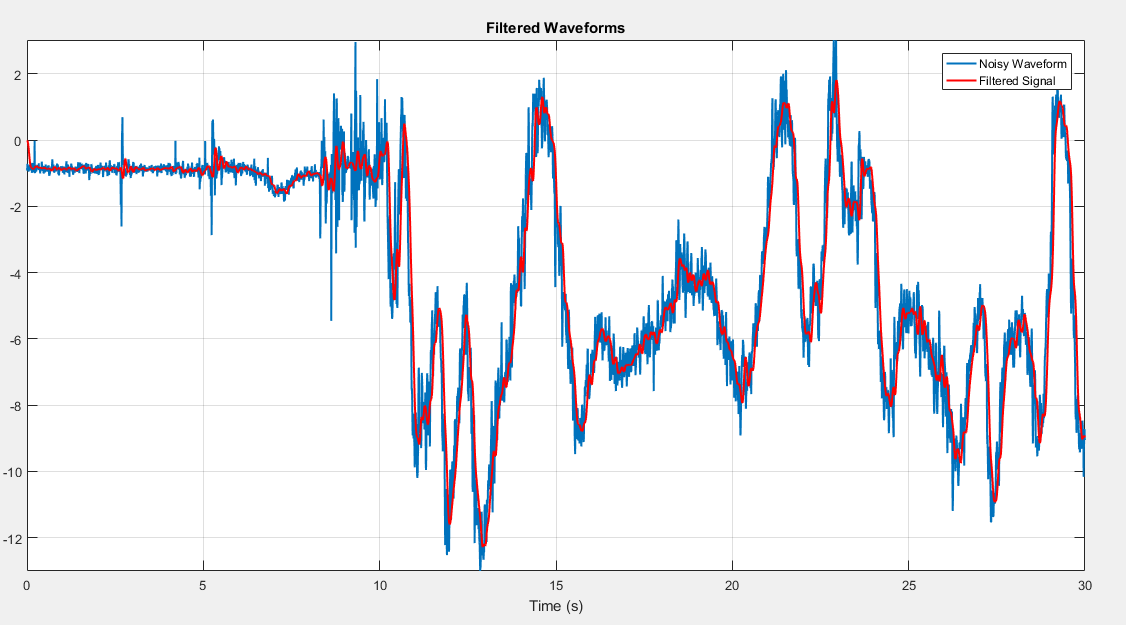
\includegraphics[width=0.5\textwidth]{images/newFilter.png}
	\caption{A Low-Pass 20th Order FIR Filter for x-axis of Accelerometer.}
	\label{newFilter}
\end{figure}

However, on top of more complex equation, the 20th order filter introduces a slight delay of about $0.1s$. For a hovering quadcopter, a tiny delay like such would carry no consequences, but a completely autonomous drone carrying out complicated tasks could suffer from such lag.
The filter part of the project could be concluded in such way - a more effective filter design is possible, but it has additional costs. The only way to know whether a stronger filter is needed is to first get the prototype completely working.

\section{Validity of tests}
It is necessary to talk about the quality of tests performed on motors and sensors. While the tools used to measure various data such as RPM and force were accurate, lack of proper documentation of the prototype's components lead to unknown expected performances. Moreover, lack of any linearities in the motor performance meant that accurate calculations could only be done around the operating range - anything beyond that point would remain an approximate, with undoubtedly increasing error.
In order to avoid such problems, it would be necessary to build a new prototype from scratch, carefully picking out required components. This would, however, require both time and money, as well as additional tools and understanding of desired performance. Overall, a longer working period would be needed to produce a prototype with better performance.

TALK ABOUT THE LACK OF COMPLETE IMPLEMENTATION AND POSSIBLE APPROACHES TO IT.